\documentclass{../mathhomework}
\usepackage{enumitem}
\usepackage{graphicx}
\usepackage{float}
\usepackage{apacite}

\newcommand{\Span}[1]{\textit{Span}\{#1\}}
\newcommand{\Vect}[1]{\pmb{#1}}
\newenvironment{Mat}{\begin{bmatrix}}{\end{bmatrix}}

% Document Settings
\topmargin=-0.45in
\evensidemargin=0in
\oddsidemargin=0in
\textwidth=6.5in
\textheight=9.0in
\headsep=0.25in

\linespread{1.5}

\setlength{\parindent}{1cm}

% Assignment Info
\newcommand{\notitleheader}{}
\coursetitle{Linear Algebra}
\courseinstructor{Professor MacArthur}

\student{Carson Storm}

\assignmenttitle{Applications of Linear Algebra in Image Processing \& Cryptography}
\assignmentduedate{September 22, 2019}

\begin{document}
\maketitle

\pagebreak

\section{Image Processing}

\subsection{Description of topic}

Digital Image Processing encompasses the transformation of digital images in order to produce an 
image that is more suitable for analysis or viewing \cite{mcconnell03}. The two main motivations for 
image processing are to change the appearance of the image and to extract information from the image, 
both rely heavily on concepts from linear algebra. Images are very often represented by matrices whose 
entries correspond to a numerical representation of the color of the pixel at the same location as 
the entry. For example, if the top left most pixel is black, if entry in the first column in the first 
row would be the number representing black. Image processing can be defined simply as performing an 
operation on the data contained in the image \cite{gonzalez18}.

Most transformations that are used for the purpose of extracting information alter the image or remove 
extraneous information until the image is in a state that is more easily analyzed. For example, an 
image can be enhanced by suppressing the details of the image that are not important to the current 
task \cite{mcconnell03}.
While altering an image is rarely enough to put an image into a state in which it is easily analyzed,
it is often a step towards the desired result. These transformations usually take the form of affine
transformation, such as scaling, reflection, translation, rotation or shearing \cite{gonzalez18}.
For example, a image may need to be flipped horizontally in order to have the right perspective
before further filtering.
The removal of extraneous information is often achieved through filtering. Filtering can take 
two main forms, spatial filter, and frequency filtering. This paper will focus on Spatial filtering, as 
it is more relevant to Linear Algebra. Spatial filter is filtering that defines a new image in terms of 
some operation that operates on each pixel in the image \cite{gonzalez18}. Some examples of spatial 
filtering are noise reduction, increasing contrast or thresholding, were if entries are not in some 
range they are set to some constant \cite{gonzalez18}. Spatial filter is performed by computing the 
discrete convolution of the image and some kernel that is specific to the type of filtering \cite{gonzalez18}. 
Convolution in the context of image processing is related to, but different than the definition of 
mathematical convolution, convolution is defined as
\begin{equation*}
    g(x,y) = \omega * f(x,y) = \sum^a_{s=-a} \sum^b_{t=-b} \omega(s,t) f(x - s, y - t)
\end{equation*}
where $g(x,y)$ is the filter image, $f(x,y)$ is the original image, $\omega$ is the kernel, such that
every entry is $(s,t)$ is of the form $-a \leq s \leq a$ and $-b \leq t \leq b$ \cite{lecarme13}.

Image processing also often used simply to alter a image for display purposes. For example, an application
might want to flip a image horizontally, so that it has the perspective we are used to, or it might want to
convert the image to grayscale. This type of image processing utilizes the same method described earlier.

\subsection{Motivation for choice of topic}

I chose the topic of image processing to discuss because I have experience implementing image processing 
algorithms, but before taking this class and researching this topic I had no idea how any of the libraries 
I was using and in most cases how each part of my algorithms functioned. I relied mostly on the documentation 
for the libraries and copying and pasting from the internet to get the algorithms to function. I was unsure why
 I was using certain method calls or why I had to transpose my matrix before passing it to a certain method.

One such time I utilized image processing in the past was for my robotics team. I needed to identify certain 
objects on the playing field and perform tasks depending on certain tasks depending on whether an object was in 
view of the camera and where it was. I had toyed with the idea of using machine learning to determine if the 
object was in view, but the time it would take to train a model and to actually use the neural network was too 
long. I instead implemented an algorithm that detected the object using computer vision, an application of image 
processing, I used various types of filtering to look for the color and shape that I knew the object would be to 
determine whether the object was in view. The process of implementing this algorithm was fairly difficult because 
I had no idea what I needed to do to get the information I needed from the camera, so I wanted to research this 
topic so that in the future if I need to implement another algorithm like this I will have a better understanding 
of what I need to do.


\subsection{Example of topic}

All of the following examples will be demonstrated by operating on Figure \ref{fig1}

\begin{figure}[H] 
    \begin{center}
        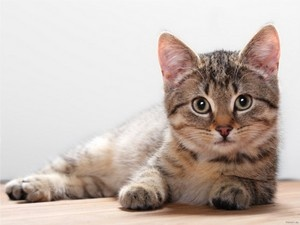
\includegraphics{figures/original.jpg}
    \end{center}
    \caption{Original Image}
    \label{fig1}
\end{figure}    

\subsubsection{Reflection}
In order to reflect an image a simple affine transformation is necessary such that every pixel in the resulting
image is defined by
\begin{equation*}
    \begin{bmatrix}
        x' \\ y'
    \end{bmatrix} =
    \begin{bmatrix}
        -1 & 0 \\
        0 & 1
    \end{bmatrix}
    \begin{bmatrix}
        x \\ y
    \end{bmatrix}
\end{equation*}
where $(x,y)$ are the pixel coordinates in the original image and $(x', y')$ are the pixel coordinates in the transformed image.
If this process performed on Figure \ref{fig1} would result in Figure \ref{fig2}.

\begin{figure}[H]
    \begin{center}
        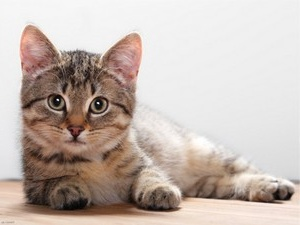
\includegraphics{figures/reflected.jpg}
    \end{center}

    \caption{Reflected image}\label{fig2}
\end{figure}

\subsubsection{Grayscale}
To convert an image to grayscale a simple operation is performed on each pixel such that each pixel in the resulting 
image is defined by
\begin{equation*}
    c = 0.3R + 0.59G + 0.11B
\end{equation*}
where $c$ is value of the pixel in the transformed image and $R,G,B$ are the red, green and blue values of the pixel in the original image.
If this process performed on Figure \ref{fig1} would result in Figure \ref{fig3}.

\begin{figure}[H]
    \begin{center}
        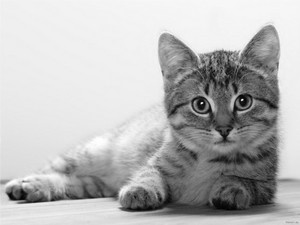
\includegraphics{figures/gray.jpg}
    \end{center}

    \caption{Grayscale image}
    \label{fig3}
\end{figure}

\subsubsection{Blur}
To blur an image, the convolution of the matrix and a Gaussian blur kernel can be computed, so that each pixel in the resulting image is defined by
\begin{equation*}
    g(x,y) = \omega * f(x,y) = \sum^1_{s=-1} \sum^1_{t=-1} \omega(s,t) f(x - s, y - t), \omega = \frac{1}{16}\begin{bmatrix}
        1 & 2 & 1 \\ 
        2 & 4 & 2 \\
        1 & 2 & 1
    \end{bmatrix}
\end{equation*}
where $g(x,y)$ is the filter image, $f(x,y)$ is the original image, $\omega$ is the Gaussian blur kernel.
If this process performed on Figure \ref{fig1} would result in Figure \ref{fig4}.

\begin{figure}[H]
    \begin{center}
        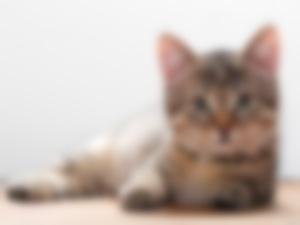
\includegraphics{figures/gaussian.jpg}
    \end{center}

    \caption{Blurred image}
    \label{fig4}
\end{figure}

\subsubsection{Laplacian}

The laplacian can be used to detect the edges in an image. To perform the laplacian on the an image, each pixel in the resulting image is defined by
\begin{equation*}
    g(x,y) = \omega * f(x,y) = \sum^1_{s=-1} \sum^1_{t=-1} \omega(s,t) f(x - s, y - t), \omega = \begin{bmatrix}
        0 & 1 & 0 \\ 
        1 & -4 & 1 \\ 
        0 & 1 & 0
    \end{bmatrix}
\end{equation*}
where $g(x,y)$ is the filter image, $f(x,y)$ is the original image, $\omega$ is the laplacian kernel.
If this process performed on Figure \ref{fig1} would result in Figure \ref{fig5}.

\begin{figure}[H]
    \begin{center}
        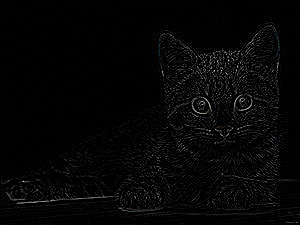
\includegraphics{figures/laplacian.jpg}
    \end{center}

    \caption{Edge detected image}
    \label{fig5}
\end{figure}

\pagebreak

\section{Cryptography}

\subsection{Description of topic}

Cryptography is a tool used to keep information that potentially untrusted entities have access to,
secret \cite{menezes97}. Cryptography is used to make this information ideally only readable by those who are 
trusted. Cryptography is based on mathematical problems are hard to solve without knowing some secret, 
and so only the person with the secret can solve the problem and read the message. Each of these problems is 
defined by a cryptosystem, which essentially defines a set of possible keys (the secret) and a set of encryption 
and decryption algorithms corresponding to each key \cite{zwicke03}. There are numerous cryptosystems that have been 
designed, but all fit into two categories, symmetric and asymmetric. A symmetric system has a shared key, that 
is used to both encrypt and decrypt the data, this means that both parties need to have the key \cite{zwicke03}. An 
asymmetric system has a public key and a private key, the public key is used to encrypt the data, and the private 
key is used to decrypt the data, this means that a key does not need to be shared with both parties \cite{zwicke03}. 
This increases the security of the system because the key of a symmetric system can be compromised when it is 
being shared. The two cryptosystems that this paper will focus on are the Hill Cipher and Lattice-based encryption 
because they are most relevant to Linear Algebra.

The Hill Cipher is a symmetric cryptosystem based on matrix multiplication \cite{overbey05}. The key for a Hill Cipher is 
an invertible matrix that is left multiplied with a matrix that represents the matrix  \cite{overbey05}. Today the Hill 
Cipher is not used do to its susceptibility to cryptoanalysis (ie. it is relatively easy to guess the key that is 
being used) \cite{overbey05}. The encryption algorithm starts by converting each character in the message to a 
standard numerical representation. Then, it places those numbers into a matrix with the same number of rows as 
the key matrix and as many columns as are needed to fit the message. This matrix is then left multiplied by the 
key which results in a matrix whose entries are the encrypted message. To decrypt the message the matrix 
containing the encrypted message is left multiplied by the inverted key. This results in a matrix whose entries 
are the numerical representation of the characters of the message \cite{hill29}.

Lattice-based encryption encompasses cryptosystems that utilize lattices in order to secure data. A lattice is the set of all linear combinations of
linearly independent vectors with integer coefficients. The lattice for the vectors $v_1, v_2, \ldots v_n$ is
\begin{equation*}
    L = \{\sum a_iv_i: a_i \in \Z\}
\end{equation*}
Most of these systems use the Shortest Vector Problem to provide a secure system.The Shortest Vector Problem relies on the 
fact that finding the shortest, non-zero vector in a lattice is hard to solve efficiently \cite{ajtai98}. These 
cryptosystems are considered to be a possible alternative to today's most popular cryptosystems for post-quantum 
cryptography since it has been shown that most of today’s leading cryptosystems can be broken by a quantum 
computer, but it has not been shown that lattice-based systems can be \cite{micciancio08}. In short, Lattice-based
cryptography utilizes concepts from Linear Algebra to create a secure cryptosystem.



\subsection{Motivation for choice of topic}

I chose cryptography because I have always been interested in cryptography, it's a perfect marriage between
math and computer science. I had never heard of Linear Algebra being involved in cryptography so I decided to
research this topic so that I could learn more about how they relate. I had heard about various other methods
of implementing cryptography, but nothing that resembled a Hill Cipher, so I was intrigued by this new approach.

Cryptography is one field that I have considered researching the future, so it has been helpful to learn about
another way that it can be implemented. While a Hill Cipher may not be very secure on its own, it can help to
improve the diffusion of other encryption algorithms, so it will be a nice tool to have in the future. 
Lattice-based encryption on the other hand seem as though they might become more popular once quantum computers
become more prevalent, so it might be very useful to have knowledge about Lattice-based encryption in the future.

Studying Lattice-based encryption has also help me to better understanding linear combinations, and how a lattice
and span relate to each other and how hard problems involving them can be to solve.

\subsection{Example of Hill Cipher}


The following piece of text "I love MATH2270" can be encrypted using a matrix by first converting the characters
of the text to numbers (in this case we will use there ascii codes).
\begin{table}[H]
    \begin{tabular}{lllllllllllllll}
    I  &    & l   & o   & v   & e   &    & M  & a  & t   & h   & 2  & 2  & 7  & 0  \\
    73 & 32 & 108 & 111 & 118 & 101 & 32 & 77 & 97 & 116 & 104 & 50 & 50 & 55 & 48
    \end{tabular}
\end{table}
\noindent If the following matrix with the following inverse is used as the cipher
\begin{equation*}
    A = \begin{bmatrix}
        1 & 2 & 3 \\
        0 & 1 & 2 \\
        0 & 0 & 5
    \end{bmatrix},
    A^{-1} = \begin{bmatrix}
        1 & -2 & \frac{1}{5} \\ 
        0 & 1 & \frac{-2}{5} \\
        0 & 0 & \frac{1}{5}
    \end{bmatrix}
\end{equation*}
Then the message can be represented by the following matrix
\begin{equation*}
    \begin{bmatrix}
        73 & 32 & 108 & 111 & 118 \\ 
        101 & 32 & 77 & 97 & 116 \\ 
        104 & 50 & 50 & 55 & 48
    \end{bmatrix}
\end{equation*}
The product of these two matrices gives use the encrypted message
\begin{equation*}
    \begin{bmatrix}
        1 & 2 & 3 \\
        0 & 1 & 2 \\
        0 & 0 & 5
    \end{bmatrix}
    \begin{bmatrix}
        73 & 32 & 108 & 111 & 118 \\ 
        101 & 32 & 77 & 97 & 116 \\ 
        104 & 50 & 50 & 55 & 48
    \end{bmatrix} = \begin{bmatrix}
        587 & 246 & 412 & 470 & 494 \\
        309 & 132 & 177 & 207 & 212 \\
        520 & 250 & 250 & 275 & 240
    \end{bmatrix}
\end{equation*}
The encrypted message is then
\begin{equation*}
    587, 246, 412, 470, 494, 309, 132, 177, 207, 212, 520, 250, 250, 275, 240
\end{equation*}
To decrypt the message, the matrix is just multiplied by the inverse of the cipher
\begin{equation*}
    \begin{bmatrix}
        1 & -2 & \frac{1}{5} \\ 
        0 & 1 & \frac{-2}{5} \\
        0 & 0 & \frac{1}{5}
    \end{bmatrix}
    \begin{bmatrix}
        587 & 246 & 412 & 470 & 494 \\
        309 & 132 & 177 & 207 & 212 \\
        520 & 250 & 250 & 275 & 240
    \end{bmatrix} =
    \begin{bmatrix}
        73 & 32 & 108 & 111 & 118 \\ 
        101 & 32 & 77 & 97 & 116 \\ 
        104 & 50 & 50 & 55 & 48
    \end{bmatrix}
\end{equation*}
This matrix can then be converted back to text to get "I love Math2270"
\begin{table}[H]
    \begin{tabular}{lllllllllllllll}
        73 & 32 & 108 & 111 & 118 & 101 & 32 & 77 & 97 & 116 & 104 & 50 & 50 & 55 & 48 \\
        I  &    & l   & o   & v   & e   &    & M  & a  & t   & h   & 2  & 2  & 7  & 0 
    \end{tabular}
\end{table}
\pagebreak

\bibliographystyle{apacite}
\bibliography{sources}

\end{document}